% =====================================================================
% Proyecto Final - Entrega 1: Diseño del esquema NoSQL y plan de implementación
% Administración de Bases de Datos - Pontificia Universidad Javeriana
%
% Cómo compilar:
%   - Overleaf: sube main.tex y er_diagram.pdf; compila con pdfLaTeX o XeLaTeX.
%   - Local:    xelatex main.tex   (o pdflatex main.tex), dos veces.
% Estilo basado en el informe del Lab 08.
% =====================================================================
\documentclass[11pt,letterpaper]{article}

\usepackage{iftex}
\ifPDFTeX
  \usepackage[utf8]{inputenc}
  \usepackage[T1]{fontenc}
  \usepackage{lmodern}
\else
  \usepackage{fontspec}
\fi
\IfFileExists{spanish.ldf}{%
  \usepackage[spanish,es-noshorthands]{babel}%
}{%
  \renewcommand{\figurename}{Figura}\renewcommand{\tablename}{Cuadro}%
}

\usepackage[margin=0.8in]{geometry}
\usepackage{microtype}
\usepackage{amssymb}
\usepackage[table]{xcolor}
\usepackage{array,booktabs}
\usepackage{enumitem}
\usepackage{graphicx,float,caption}
\usepackage{listings}
\usepackage{titlesec}
\usepackage[colorlinks=true,linkcolor=blue,urlcolor=blue,citecolor=blue,
            pdftitle={Proyecto Final - Entrega 1: Esquema NoSQL y plan de implementación},
            pdfauthor={Samuel Tovar, Juan Romero, Carlos Pinzón Caicedo, Alejandro Padilla Gaviria}]{hyperref}

% ----- formato general (estilo Lab 08)
\setlength{\emergencystretch}{3em}
\setlist[itemize]{label=\raisebox{0.25ex}{\tiny$\blacksquare$},itemsep=4pt,topsep=5pt}
\setlist[enumerate]{itemsep=4pt,topsep=5pt}
\titleformat{\section}{\normalfont\Large\bfseries}{\thesection.}{1em}{}
\titleformat{\subsection}{\normalfont\large\bfseries}{\thesubsection.}{1em}{}
\titlespacing*{\section}{0pt}{16pt}{8pt}
\titlespacing*{\subsection}{0pt}{12pt}{6pt}
\captionsetup{labelsep=colon}

% ----- columnas de tabla con ancho relativo
\newcolumntype{Y}[1]{>{\raggedright\arraybackslash}p{\dimexpr #1\linewidth-2\tabcolsep\relax}}

% ----- listados de código (fondo gris, números de línea, comentarios en azul)
\definecolor{codebg}{gray}{0.96}
\definecolor{codecomment}{HTML}{2F5D8C}
\definecolor{codestring}{HTML}{C00000}
\definecolor{codekeyword}{HTML}{007F00}
\lstdefinelanguage{mongosh}{
  morekeywords={const,let,var,function,return,true,false,null},
  morecomment=[l]{//},
  morestring=[b]",
  sensitive=true}
\lstdefinelanguage{tree}{morecomment=[l]{\#}}
\lstdefinestyle{lab}{
  basicstyle=\fontsize{7}{8.6}\selectfont\ttfamily,
  backgroundcolor=\color{codebg},
  numbers=left, numberstyle=\fontsize{5}{6}\selectfont\color{gray}, numbersep=7pt,
  commentstyle=\itshape\color{codecomment},
  keywordstyle=\color{codekeyword},
  stringstyle=\color{codestring},
  showstringspaces=false, breaklines=true, keepspaces=true,
  frame=single, framerule=0pt, rulecolor=\color{codebg}, framesep=5pt,
  xleftmargin=14pt, xrightmargin=0pt,
  aboveskip=8pt, belowskip=8pt,
  extendedchars=true,
  literate={á}{{\'a}}1 {é}{{\'e}}1 {í}{{\'i}}1 {ó}{{\'o}}1 {ú}{{\'u}}1
           {Á}{{\'A}}1 {É}{{\'E}}1 {Í}{{\'I}}1 {Ó}{{\'O}}1 {Ú}{{\'U}}1
           {ñ}{{\~n}}1 {Ñ}{{\~N}}1 {ü}{{\"u}}1 {¿}{{?`}}1 {¡}{{!`}}1}

% ----- caja que evita que un listado se parta entre páginas
\newenvironment{codebox}{\par\noindent\begin{minipage}{\linewidth}}{\end{minipage}\par}

\begin{document}

% ===================================================================== TÍTULO
\vspace*{0.4in}
\begin{center}
  {\Large Administración de Bases de Datos\par}
  {\Large Proyecto Final: Potencial Solar de Techos en Municipios PDET\par}
  {\large Entrega 1: Diseño del Esquema NoSQL y Plan de Implementación\par}
  \vspace{1.2em}
  {\large \begin{tabular}[t]{c@{\hspace{4em}}c}
     Samuel Tovar & Juan Romero \\[0.3em]
     Carlos Pinzón Caicedo & Alejandro Padilla Gaviria
   \end{tabular}\par}
  {\large Pontificia Universidad Javeriana\par}
  \vspace{0.8em}
  {\large 2 de noviembre de 2026\par}
\end{center}

% ===================================================================== 1
\section{Introducción}

Este informe presenta la primera entrega del proyecto final de Administración de Bases de Datos:
el diseño del esquema NoSQL y el plan de implementación para estimar el potencial solar de los
techos en los municipios PDET (Programas de Desarrollo con Enfoque Territorial), tal como lo solicita
la Oficina de Investigación e Información de la Unidad de Planeación Minero Energética (UPME). Su
objetivo es fijar la tecnología, las fuentes de datos, el modelo de datos (diagrama E-R y
diccionario) y el plan de trabajo de las entregas 2 a 5.

La UPME busca identificar municipios donde desplegar pruebas de concepto de energía solar. El
criterio de priorización son los territorios PDET (170 municipios agrupados en 16 subregiones): a
mayor área de techos aprovechables, mayor potencial de captación solar. El proyecto debe contar las
edificaciones y estimar el área total de techos aptos por municipio PDET, con una solución NoSQL y
comparando al menos dos conjuntos de datos abiertos de huellas de edificios.

Los archivos del proyecto (este PDF, su fuente en \LaTeX{}, el diagrama E-R, el archivo
\texttt{docker-compose.yml} y los parámetros) se entregan en el repositorio
\url{https://github.com/SamT81/Proyecto-ABD}.

% ===================================================================== 2
\section{Selección y Descripción de las Fuentes de Datos}

\begin{itemize}
  \item \textbf{Microsoft Building Footprints} (seleccionada). Huellas de edificios derivadas de
  imágenes de Bing Maps (2014--2021, con fuentes como Maxar y Airbus), con más de 999 millones de
  detecciones en el mundo. Licencia ODbL. Fuente:
  \url{https://planetarycomputer.microsoft.com/dataset/ms-buildings}. Aporta la geometría del
  edificio; el área se calcula en el ETL.

  \item \textbf{Google Open Buildings} (seleccionada). 1800 millones de detecciones en 58 millones
  de km$^2$ (África, Asia del Sur y del Sudeste, América Latina y el Caribe), en su tercera versión.
  Licencias CC BY 4.0 y ODbL v1.0. Fuente: \url{https://sites.research.google/gr/open-buildings/}.
  Incluye el área (\texttt{area\_in\_meters}) y un puntaje de confianza por edificio.

  \item \textbf{GlobalBuildingAtlas, TUM} (no seleccionada). 2750 millones de modelos de edificios
  a partir de imágenes de 2019, con resolución de $3\times3$ m y modelos 3D. Licencia MIT con
  \emph{Commons Clause}. Fuente: \url{https://github.com/zhu-xlab/GlobalBuildingAtlas}. Excede el
  mínimo de dos fuentes y su valor agregado (altura 3D) no es necesario para estimar el área de
  techo; queda como extensión opcional.

  \item \textbf{DANE, Marco Geoestadístico Nacional (MGN) 2025.} Límites administrativos de
  Colombia en todos los niveles geográficos (ZIP de 1.5 GB). Se extrae la capa municipal. Fuente:
  \url{https://geoportal.dane.gov.co/}.

  \item \textbf{Lista de municipios PDET.} 170 municipios en 16 subregiones, según la Agencia de
  Renovación del Territorio (Decreto 893 de 2017). Se usa para filtrar la capa municipal del MGN por
  código DIVIPOLA de 5 dígitos.
\end{itemize}

% ===================================================================== 3
\section{Metodología}

\subsection{Herramientas}

\begin{itemize}
  \item \textbf{MongoDB} (Community Server, en Docker): almacén de documentos con soporte nativo de
  GeoJSON, índices \texttt{2dsphere}, operadores \texttt{\$geoWithin} y \texttt{\$geoIntersects} y
  \emph{aggregation pipeline}.
  \item \textbf{Python} con \texttt{geopandas}, \texttt{pyarrow} y \texttt{pymongo} para el ETL:
  lectura por partes, reparación de geometrías, reproyección y carga.
  \item \textbf{Docker Compose} para levantar la base de datos de forma reproducible.
  \item \textbf{QGIS} o \textbf{MongoDB Compass} para validar visualmente geometrías e índices.
\end{itemize}

\subsection{Decisiones clave}

El Cuadro~\ref{tab:decisiones} resume las decisiones de diseño y su justificación.

\begin{table}[!htbp]
\centering\small
\renewcommand{\arraystretch}{1.1}
\begin{tabular}{Y{0.17}Y{0.28}Y{0.55}}
\toprule
Decisión & Elección & Justificación \\
\midrule
Motor NoSQL
  & \textbf{MongoDB} (almacén de documentos, Community Server en Docker)
  & Soporte nativo de GeoJSON, índices \texttt{2dsphere}, operadores \texttt{\$geoWithin} /
    \texttt{\$geoIntersects} y \emph{aggregation pipeline} para agrupar por municipio. Cliente
    Python (\texttt{pymongo}) maduro y esquema flexible para atributos distintos por fuente. \\
\addlinespace[3pt]
Datasets (mínimo 2)
  & \textbf{Microsoft Building Footprints} y \textbf{Google Open Buildings}
  & Ambos cubren Colombia. Google incluye área y confianza; Microsoft aporta la geometría y el área
    se calcula, lo que hace interesante la comparación. Formatos distintos (GeoParquet/GeoJSON
    frente a CSV) exigen un ETL robusto. \\
\addlinespace[3pt]
Fronteras
  & \textbf{DANE MGN 2025}, nivel municipal, filtrado a los 170 municipios PDET
  & Fuente oficial. La lista PDET se toma de la Agencia de Renovación del Territorio (Decreto 893 de
    2017) y se cruza por código DIVIPOLA de 5 dígitos. \\
\addlinespace[3pt]
Sistema de coordenadas
  & Almacenamiento en \textbf{EPSG:4326}; áreas en \textbf{EPSG:9377}
  & \texttt{2dsphere} requiere longitud/latitud en WGS84. Calcular áreas en grados no es válido;
    MAGNA-SIRGAS Origen Nacional (EPSG:9377) es el CRS proyectado oficial para Colombia. \\
\addlinespace[3pt]
Edificio $\rightarrow$ municipio
  & \texttt{municipality\_code} \textbf{pre-asignado en el ETL} con el punto representativo del
    edificio
  & Evita doble conteo en los límites y permite agregar con un índice simple, sin join espacial en
    cada consulta. \texttt{\$geoWithin} se usa para validación cruzada. \\
\addlinespace[3pt]
Techo ``apto''
  & Criterio \textbf{parametrizable}: \texttt{area\_m2} $\geq A_{\min}$ y, en Google,
    \texttt{confidence} $\geq C_{\min}$
  & Valores iniciales a calibrar en el EDA (por ejemplo $A_{\min}=15$ m$^2$, $C_{\min}=0.70$). Se
    guardan en \texttt{results.params} para que cada resultado sea trazable. \\
\bottomrule
\end{tabular}
\caption{Decisiones clave de diseño y su justificación.}
\label{tab:decisiones}
\end{table}

\subsection{Pasos}

\begin{enumerate}
  \item \textbf{Validar y reparar:} las geometrías se reparan con \texttt{make\_valid}; las
  irrecuperables se descartan y se cuentan en \texttt{ingestion\_log}.
  \item \textbf{Calcular el área} en EPSG:9377: Microsoft se calcula; en Google se conserva
  \texttt{area\_in\_meters} original y se contrasta con el área recalculada en una muestra para
  verificar consistencia.
  \item \textbf{Asignar municipio} con un join espacial entre el punto representativo del edificio y
  los polígonos PDET; los edificios fuera de PDET se descartan antes de insertar.
  \item \textbf{Agregar} por (\texttt{municipality\_code}, \texttt{source}): total de edificios, área
  total y área apta según los parámetros; el resultado se guarda en \texttt{results} junto con
  \texttt{params} y \texttt{computed\_at}.
  \item \textbf{Comparar fuentes:} diferencia absoluta y relativa de conteo y área por municipio,
  correlación y municipios con mayores discrepancias; ranking de municipios por área apta.
  \item \textbf{Visualizar:} mapas coropléticos y tablas de los primeros $N$ municipios.
\end{enumerate}

\subsection{Flujo general}

\begin{codebox}\begin{lstlisting}[style=lab,numbers=none,language={}]
[DANE MGN 2025] ----+
[Lista PDET (ART)] -+--> ETL Python (geopandas) --> municipalities  (2dsphere)

[Microsoft GeoParquet/GeoJSON] --> ETL por lotes --> buildings_microsoft (2dsphere)
[Google CSV.gz (celdas S2)]    --> ETL por lotes --> buildings_google    (2dsphere)
                                        |
                                        v
              Aggregation pipeline ($group por municipality_code)
                                        |
                                        v
              results --> tablas y mapas (geopandas, matplotlib) --> informe final
\end{lstlisting}\end{codebox}

\subsection{Fases y entregables}

El Cuadro~\ref{tab:fases} asocia cada semana con su entrega y su producto.

\begin{table}[!htbp]
\centering\small
\renewcommand{\arraystretch}{1.1}
\begin{tabular}{Y{0.09}Y{0.19}Y{0.50}Y{0.22}}
\toprule
Semana & Entrega & Actividades principales & Producto \\
\midrule
1 & Esquema NoSQL y plan
  & Selección de tecnología y datasets; diseño E-R; diccionario de datos; plan; repositorio base
    (README, \texttt{docker-compose}).
  & Este documento y repositorio inicial \\
\addlinespace[3pt]
2 & Fronteras PDET
  & Descarga del MGN2025 (ZIP de 1.5 GB) y verificación (\emph{checksum}, CRS, conteo = 170
    municipios); filtrado PDET; reparación de geometrías; carga en \texttt{municipalities}; índice
    \texttt{2dsphere}.
  & Colección \texttt{municipalities}, bitácora de calidad \\
\addlinespace[3pt]
3 & Huellas de edificios
  & Descarga solo de las particiones que intersectan PDET; carga por lotes con pre-asignación de
    municipio; índices; EDA (conteos, distribución de áreas, confianza, geometrías inválidas).
  & \texttt{buildings\_microsoft}, \texttt{buildings\_google}, EDA \\
\addlinespace[3pt]
4 & Análisis y reporte final
  & Agregación por municipio y fuente; comparación entre fuentes; tablas y mapas coropléticos;
    informe técnico con discusión y recomendaciones; defensa.
  & \texttt{results}, mapas, informe final \\
\bottomrule
\end{tabular}
\caption{Fases del proyecto y entregables asociados.}
\label{tab:fases}
\end{table}

\subsection{Manejo de grandes volúmenes}

\begin{itemize}
  \item \textbf{Filtrar en origen:} descargar solo archivos o celdas que intersecten la caja
  envolvente de los municipios PDET.
  \item \textbf{Lectura por partes} (\emph{chunks} o \emph{row groups} de Parquet); nunca cargar un
  archivo completo en memoria.
  \item \textbf{Inserción masiva:} \texttt{insert\_many(ordered=False)} en lotes de 10\,000 a
  50\,000 documentos y procesamiento en paralelo por archivo.
  \item \textbf{Índices después de la carga:} crear \texttt{2dsphere} y los demás índices al
  terminar la inserción, que es más rápido que mantenerlos durante la carga.
  \item \textbf{Carga idempotente y reanudable:} \texttt{ingestion\_log} guarda \emph{checksum} y
  conteos por archivo, de modo que un archivo ya cargado no se duplica.
  \item \textbf{Menos bytes por documento:} solo los campos necesarios y coordenadas con 6
  decimales ($\approx$0.1 m).
\end{itemize}

\subsection{Reproducibilidad}

\begin{codebox}\begin{lstlisting}[style=lab,numbers=none,language=tree]
repo/
  README.md              # pasos de ejecución de punta a punta
  docker-compose.yml     # MongoDB (y mongo-express opcional)
  requirements.txt       # dependencias con versiones fijas
  config/params.yaml     # rutas, CRS, A_min, C_min, tamaño de lote
  src/
    01_load_municipalities.py
    02_load_buildings.py
    03_compute_results.py
    04_make_maps.py
  docs/                  # PDFs de cada entrega, fuente del E-R (.dot) e imagen
  data/                  # ignorado por git; se documentan URLs y checksums
  notebooks/             # EDA
\end{lstlisting}\end{codebox}

\begin{itemize}
  \item Scripts numerados e idempotentes; un solo comando levanta la base de datos con Docker.
  \item Los datos no se versionan: el README documenta URL de descarga, fecha y \emph{checksum} de
  cada fuente.
  \item Se respeta la atribución exigida por las licencias (ODbL y CC BY 4.0) en mapas e informe.
\end{itemize}

% ===================================================================== 4
\section{Diseño del Esquema y Modelado de Datos}

\subsection{Diagrama E-R}

La Figura~\ref{fig:er} muestra el diagrama E-R de las cinco colecciones.

\begin{figure}[!tbp]
  \centering
  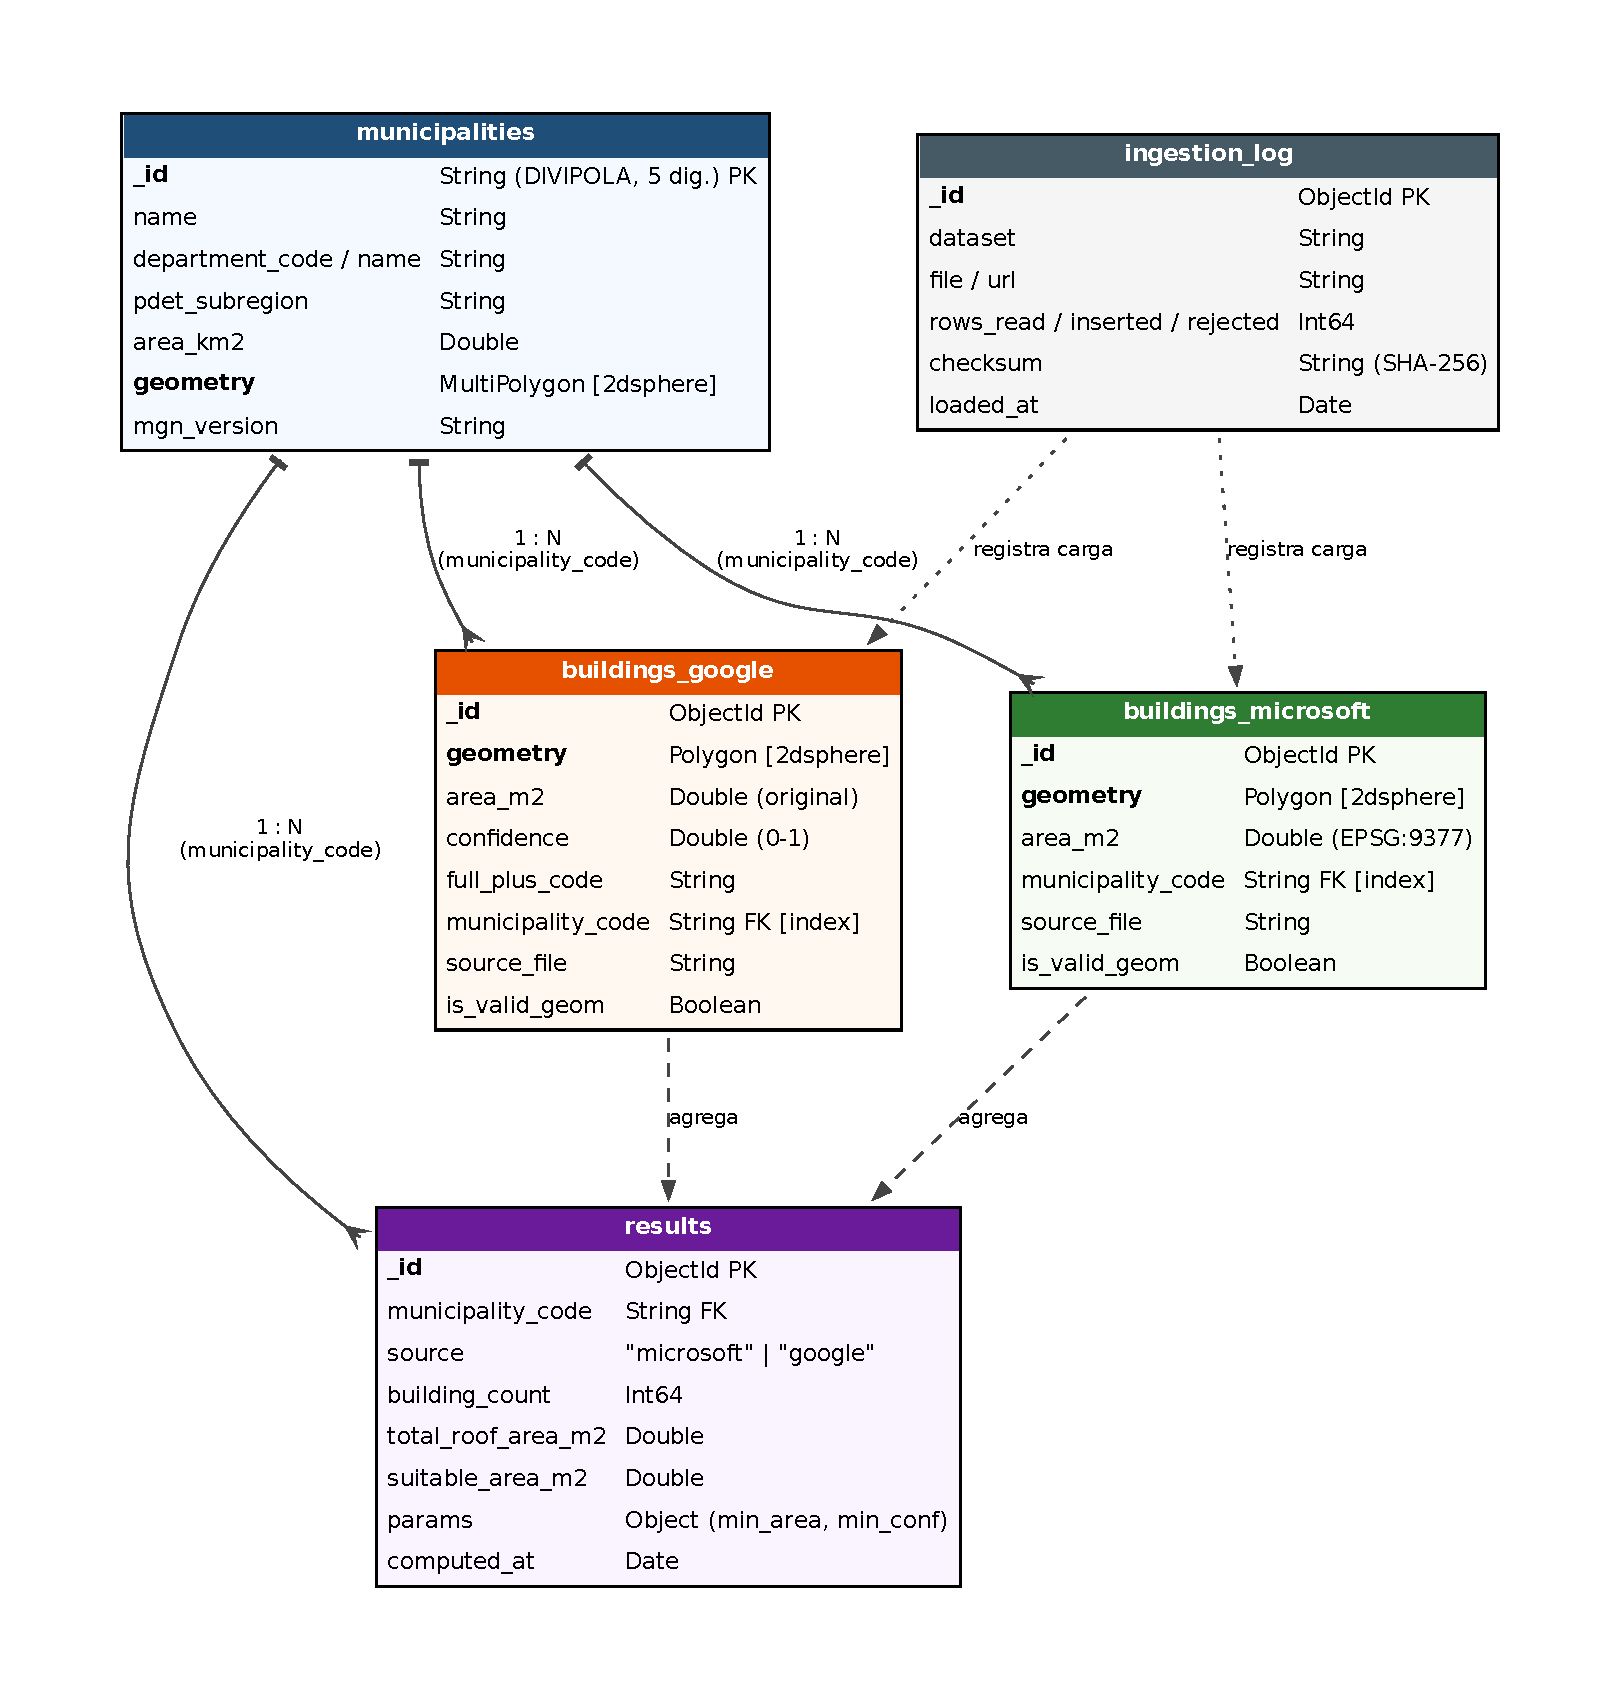
\includegraphics[height=0.78\textheight,width=\linewidth,keepaspectratio]{er_diagram.pdf}
  \caption{Diagrama E-R de las colecciones (PK: clave primaria, FK: clave lógica, [2dsphere] y
  [index]: índices). Cardinalidad 1:N en notación de pata de gallo.}
  \label{fig:er}
\end{figure}

\subsection{Principios de diseño}

\begin{itemize}
  \item \textbf{Referenciar, no embeber:} un municipio tiene desde miles hasta cientos de miles de
  edificios; embeberlos superaría el límite de 16 MB por documento y haría ineficientes las
  actualizaciones.
  \item \textbf{Una colección por fuente:} los atributos y la calidad son distintos
  (\texttt{confidence} solo existe en Google). Así se comparan las fuentes y se recarga una sin
  afectar la otra.
  \item \textbf{Desnormalizar \texttt{municipality\_code} en cada edificio:} cuesta pocos bytes por
  documento y evita un join espacial en cada agregación.
  \item \textbf{Resultados materializados:} \texttt{results} guarda cada cálculo con sus parámetros
  y fecha, lo que facilita mapas, tablas y la auditoría.
  \item \textbf{Claves lógicas:} MongoDB no impone claves foráneas; \texttt{municipality\_code}
  referencia a \texttt{municipalities.\_id} por convención y se valida en el ETL.
\end{itemize}

\subsection{Diccionario de datos}

Los Cuadros~\ref{tab:dd-mun} a~\ref{tab:dd-log} describen los campos de cada colección. Los nombres
exactos de los campos del MGN (códigos y nombres) se confirman en la Entrega 2 sobre la capa
descargada.

\begin{table}[!htbp]
\centering\small
\renewcommand{\arraystretch}{1.1}
\begin{tabular}{Y{0.23}Y{0.20}Y{0.07}Y{0.50}}
\toprule
Campo & Tipo & Req. & Descripción \\
\midrule
\texttt{\_id} & String & Sí & Código DIVIPOLA de 5 dígitos (2 de departamento + 3 de municipio),
  p.\,ej. ``05045''. \\
\texttt{name} & String & Sí & Nombre del municipio (campo de nombre de la capa MGN). \\
\texttt{department\_code} & String & Sí & Código de departamento, 2 dígitos. \\
\texttt{department\_name} & String & Sí & Nombre del departamento. \\
\texttt{pdet\_subregion} & String & Sí & Subregión PDET (una de 16), según la lista de la ART. \\
\texttt{area\_km2} & Double & Sí & Área calculada en EPSG:9377. \\
\texttt{geometry} & GeoJSON MultiPolygon & Sí & Límite municipal en WGS84. Índice
  \texttt{2dsphere}. \\
\texttt{mgn\_version} & String & Sí & Versión del MGN usada (p.\,ej. ``MGN2025''). \\
\bottomrule
\end{tabular}
\caption{Diccionario de datos de la colección \texttt{municipalities} (límites municipales PDET,
DANE MGN).}
\label{tab:dd-mun}
\end{table}

\begin{table}[!htbp]
\centering\small
\renewcommand{\arraystretch}{1.1}
\begin{tabular}{Y{0.23}Y{0.20}Y{0.07}Y{0.50}}
\toprule
Campo & Tipo & Req. & Descripción \\
\midrule
\texttt{\_id} & ObjectId & Sí & Identificador del documento. \\
\texttt{geometry} & GeoJSON Polygon & Sí & Huella del edificio en WGS84. Índice \texttt{2dsphere}. \\
\texttt{area\_m2} & Double & Sí & Área calculada en EPSG:9377. \\
\texttt{municipality\_code} & String (FK) & Sí & Referencia a \texttt{municipalities.\_id}.
  Indexado. \\
\texttt{source\_file} & String & Sí & Archivo o partición de origen (trazabilidad). \\
\texttt{is\_valid\_geom} & Boolean & Sí & \texttt{false} si la geometría original era inválida y se
  reparó. \\
\bottomrule
\end{tabular}
\caption{Diccionario de datos de la colección \texttt{buildings\_microsoft} (huellas de Microsoft
dentro de PDET).}
\label{tab:dd-ms}
\end{table}

\begin{table}[!htbp]
\centering\small
\renewcommand{\arraystretch}{1.1}
\begin{tabular}{Y{0.23}Y{0.20}Y{0.07}Y{0.50}}
\toprule
Campo & Tipo & Req. & Descripción \\
\midrule
\texttt{\_id} & ObjectId & Sí & Identificador del documento. \\
\texttt{geometry} & GeoJSON Polygon & Sí & Huella en WGS84 (convertida desde WKT). Índice
  \texttt{2dsphere}. \\
\texttt{area\_m2} & Double & Sí & Área original de la fuente (\texttt{area\_in\_meters}). \\
\texttt{confidence} & Double & Sí & Puntaje de confianza del modelo (0 a 1). \\
\texttt{full\_plus\_code} & String & No & Plus Code de la fuente. \\
\texttt{municipality\_code} & String (FK) & Sí & Referencia a \texttt{municipalities.\_id}.
  Indexado. \\
\texttt{source\_file} & String & Sí & Archivo o celda S2 de origen. \\
\texttt{is\_valid\_geom} & Boolean & Sí & \texttt{false} si la geometría original era inválida y se
  reparó. \\
\bottomrule
\end{tabular}
\caption{Diccionario de datos de la colección \texttt{buildings\_google} (huellas de Google Open
Buildings dentro de PDET).}
\label{tab:dd-goog}
\end{table}

\begin{table}[!htbp]
\centering\small
\renewcommand{\arraystretch}{1.1}
\begin{tabular}{Y{0.23}Y{0.20}Y{0.07}Y{0.50}}
\toprule
Campo & Tipo & Req. & Descripción \\
\midrule
\texttt{\_id} & ObjectId & Sí & Identificador del documento. \\
\texttt{municipality\_code} & String (FK) & Sí & Referencia a \texttt{municipalities.\_id}. \\
\texttt{source} & String & Sí & ``microsoft'' o ``google''. \\
\texttt{building\_count} & Int64 & Sí & Total de edificios detectados en el municipio. \\
\texttt{total\_roof\_area\_m2} & Double & Sí & Suma de \texttt{area\_m2} de todos los edificios. \\
\texttt{suitable\_area\_m2} & Double & Sí & Suma de \texttt{area\_m2} de los edificios que cumplen el
  criterio de techo apto. \\
\texttt{params} & Object & Sí & Parámetros usados: \texttt{min\_area\_m2}, \texttt{min\_confidence},
  CRS del área. \\
\texttt{computed\_at} & Date & Sí & Fecha y hora del cálculo. \\
\bottomrule
\end{tabular}
\caption{Diccionario de datos de la colección \texttt{results} (métricas por municipio y fuente; se
llena en la Entrega 4).}
\label{tab:dd-res}
\end{table}

\begin{table}[!htbp]
\centering\small
\renewcommand{\arraystretch}{1.1}
\begin{tabular}{Y{0.23}Y{0.20}Y{0.07}Y{0.50}}
\toprule
Campo & Tipo & Req. & Descripción \\
\midrule
\texttt{\_id} & ObjectId & Sí & Identificador del documento. \\
\texttt{dataset} & String & Sí & ``mgn2025'', ``microsoft'' o ``google''. \\
\texttt{file} & String & Sí & Archivo o URL de origen. \\
\texttt{rows\_read} & Int64 & Sí & Registros leídos. \\
\texttt{rows\_inserted} & Int64 & Sí & Registros insertados. \\
\texttt{rows\_rejected} & Int64 & Sí & Registros descartados (geometría irrecuperable o fuera de
  PDET). \\
\texttt{checksum} & String & Sí & SHA-256 del archivo de origen. \\
\texttt{loaded\_at} & Date & Sí & Fecha y hora de la carga. \\
\bottomrule
\end{tabular}
\caption{Diccionario de datos de la colección \texttt{ingestion\_log} (bitácora de cargas: calidad y
reproducibilidad).}
\label{tab:dd-log}
\end{table}

\subsection{Índices}

El Cuadro~\ref{tab:indices} lista los índices por colección y el siguiente listado muestra cómo
crear los principales.

\begin{table}[!htbp]
\centering\small
\renewcommand{\arraystretch}{1.1}
\begin{tabular}{Y{0.30}Y{0.38}Y{0.32}}
\toprule
Colección & Índice & Propósito \\
\midrule
\texttt{municipalities} & \texttt{\{ geometry: "2dsphere" \}}
  & Consultas espaciales y asignación de municipio. \\
\texttt{municipalities} & \texttt{\{ pdet\_subregion: 1 \}} & Agrupar y filtrar por subregión. \\
\texttt{buildings\_microsoft}, \texttt{buildings\_google} & \texttt{\{ geometry: "2dsphere" \}}
  & Consultas espaciales (\texttt{\$geoWithin}, \texttt{\$geoIntersects}). \\
\texttt{buildings\_microsoft}, \texttt{buildings\_google}
  & \texttt{\{ municipality\_code: 1, area\_m2: 1 \}}
  & Agregación por municipio y filtro por área. \\
\texttt{buildings\_google} & \texttt{\{ confidence: 1 \}} & Filtro por umbral de confianza. \\
\texttt{results} & \texttt{\{ municipality\_code: 1, source: 1, computed\_at: -1 \}}
  & Última corrida por municipio y fuente. \\
\bottomrule
\end{tabular}
\caption{Índices por colección.}
\label{tab:indices}
\end{table}

\begin{codebox}\begin{lstlisting}[style=lab,language=mongosh]
db.municipalities.createIndex({ geometry: "2dsphere" })
db.buildings_google.createIndex({ geometry: "2dsphere" })
db.buildings_google.createIndex({ municipality_code: 1, area_m2: 1 })
\end{lstlisting}\end{codebox}

% ===================================================================== 5
\section{Análisis: Ejemplos de Documentos y Consultas}

\subsection{Ejemplos de documentos}

Los siguientes documentos son ilustrativos (los valores no provienen de los datos reales).

\begin{codebox}\begin{lstlisting}[style=lab,language=mongosh]
// municipalities
{
  "_id": "05045",
  "name": "Apartadó",
  "department_code": "05",
  "department_name": "Antioquia",
  "pdet_subregion": "Urabá antioqueño",
  "area_km2": <double>,
  "geometry": { "type": "MultiPolygon", "coordinates": [ ... ] },
  "mgn_version": "MGN2025"
}
\end{lstlisting}\end{codebox}

\begin{codebox}\begin{lstlisting}[style=lab,language=mongosh]
// buildings_google
{
  "geometry": { "type": "Polygon", "coordinates": [[[-76.63, 7.88], ... ]] },
  "area_m2": 85.3,
  "confidence": 0.87,
  "full_plus_code": "<plus code>",
  "municipality_code": "05045",
  "source_file": "<celda S2>.csv.gz",
  "is_valid_geom": true
}
\end{lstlisting}\end{codebox}

\subsection{Consultas de ejemplo}

\begin{codebox}\begin{lstlisting}[style=lab,language=mongosh]
// 1. Conteo y área por municipio con criterio de techo apto (Google)
db.buildings_google.aggregate([
  { $match: { confidence: { $gte: 0.70 }, area_m2: { $gte: 15 } } },
  { $group: { _id: "$municipality_code",
              n: { $sum: 1 }, area_m2: { $sum: "$area_m2" } } },
  { $sort: { area_m2: -1 } }
])

// 2. Validación cruzada: edificios dentro de un municipio (consulta espacial)
const m = db.municipalities.findOne({ _id: "05045" });
db.buildings_microsoft.countDocuments(
  { geometry: { $geoWithin: { $geometry: m.geometry } } })
\end{lstlisting}\end{codebox}

\noindent\textbf{Discusión de las decisiones clave.}
\begin{itemize}
  \item La consulta 1 agrupa por \texttt{municipality\_code} sin ningún join espacial gracias a la
  pre-asignación hecha en el ETL; el \texttt{\$match} aplica el criterio de techo apto, cuyos
  umbrales son parámetros.
  \item La consulta 2 usa \texttt{\$geoWithin} con el polígono municipal para validar la
  pre-asignación. Los conteos pueden diferir ligeramente en los edificios que cruzan el límite
  municipal, porque la asignación usa el punto representativo y \texttt{\$geoWithin} exige que el
  edificio completo quede dentro del polígono.
  \item En la Entrega 4 los resultados de la consulta 1 se materializan en \texttt{results} con
  \texttt{\$merge}.
\end{itemize}

% ===================================================================== 6
\section{Conclusiones y Limitaciones}

\begin{itemize}
  \item El esquema separa las fuentes de los resultados, referencia los municipios por código
  DIVIPOLA y permite comparar Microsoft y Google sobre los mismos municipios PDET. MongoDB cubre las
  operaciones espaciales y las agregaciones que exige el proyecto.
  \item El criterio de techo apto es un supuesto metodológico: sus valores iniciales
  ($A_{\min}=15$ m$^2$, $C_{\min}=0.70$) se calibran en el EDA de la Entrega 3 y quedan guardados
  con cada resultado.
  \item Los nombres exactos de los campos del MGN y la cobertura de ambas fuentes sobre los 170
  municipios PDET se verifican en las entregas 2 y 3; hasta entonces son supuestos del diseño.
  \item Los siguientes pasos son cargar las fronteras PDET con su índice \texttt{2dsphere}
  (Entrega 2) y cargar las huellas de edificios por lotes (Entrega 3).
\end{itemize}

El Cuadro~\ref{tab:riesgos} resume los riesgos identificados y su mitigación.

\begin{table}[!htbp]
\centering\small
\renewcommand{\arraystretch}{1.1}
\begin{tabular}{Y{0.38}Y{0.62}}
\toprule
Riesgo & Mitigación \\
\midrule
Volumen y tiempo de descarga o carga
  & Filtrado en origen, lotes, paralelismo y empezar la descarga desde la semana 1. \\
\addlinespace[3pt]
Geometrías inválidas rechazadas por \texttt{2dsphere}
  & \texttt{make\_valid} en el ETL y registro en \texttt{ingestion\_log}. \\
\addlinespace[3pt]
Municipios PDET mal identificados (versión del MGN o códigos)
  & Cruce por código DIVIPOLA de 5 dígitos y verificación de que el resultado sean 170
    municipios. \\
\addlinespace[3pt]
Polígonos municipales muy detallados (límite de 16 MB por documento, rendimiento)
  & Verificar tamaño al cargar; si hace falta, usar una versión simplificada solo para
    visualización y conservar la original. \\
\addlinespace[3pt]
Duplicados o traslapes dentro de una fuente; fechas de captura distintas entre fuentes
  & Se reportan en el EDA; las fuentes no se fusionan, se comparan por municipio. \\
\addlinespace[3pt]
Carga de trabajo desigual en el equipo
  & Reparto por entregable y commits de ambos integrantes en cada entrega. \\
\bottomrule
\end{tabular}
\caption{Riesgos y mitigaciones.}
\label{tab:riesgos}
\end{table}

\bigskip
\noindent\textbf{Referencias.} Microsoft, \emph{Microsoft Building Footprints} (Planetary Computer).
Google Research, \emph{Open Buildings}, versión 3. Technical University of Munich,
\emph{GlobalBuildingAtlas}. DANE, \emph{Marco Geoestadístico Nacional (MGN) 2025}. Agencia de
Renovación del Territorio, ``¿Qué son los PDET?''. Calderón Romero, A.\,O., enunciado del proyecto
final de Administración de Bases de Datos (25 de octubre de 2026).

\end{document}
